This chapter explains the dynamic model derivation of the soft robotic manipulator. Forward kinematics describe the robots configuration for a given set of initial conditions. These derived forward kinematics allows to derive a dynamic model 

\section{Kinematics}

The soft actuator studied in this thesis is shown in Figure \ref{fig2:kinematicschematic}. It consists of two bellows placed in parallel. The outside of the bellows are connected, forming the centre line of the actuator. Furthermore, the bellows are connected by a flange at the top and bottom. The soft robot is pneumatically actuated using air pumps. Each bellow can be inflated individually via a hole at one end of the actuator. This flange will be fixed to the ground. The other end is closed, allowing to pressurize the bellows. The actuators geometry and material choice allows the bellows to extend when pressurized. Since each bellow can be inflated independently, the entire actuator can increase its length and change orientation. The actuator is actuated in a single plane, hence the name planar soft actuator. Undesired out of plane motions are deemed negligibly small.

  \begin{minipage}{\linewidth}
      \centering
      \begin{minipage}{0.45\linewidth}
        \begin{figure}[H]
        \centering
            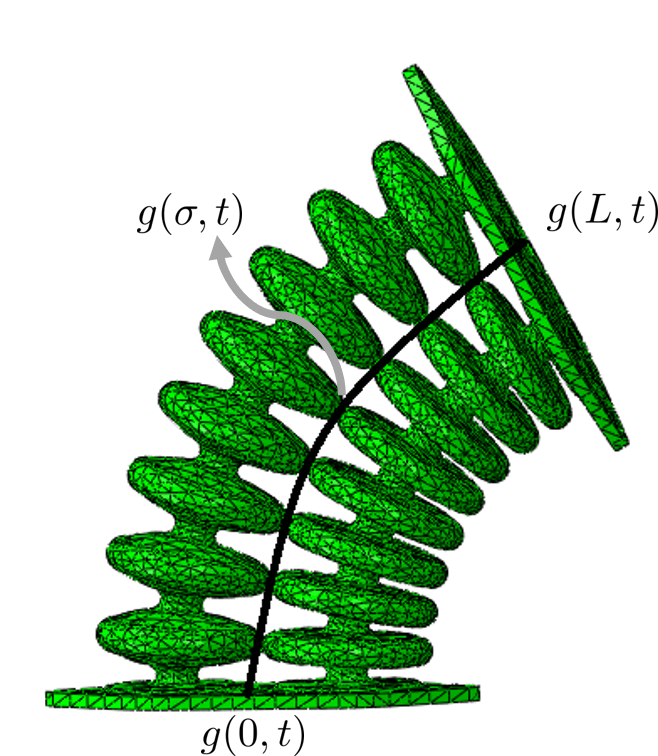
\includegraphics[width=\textwidth]{Figures/Chapter2/schematickinematic.png}
            \caption{Planar soft actuator with the backbone curve $g(\sigma,t)$.}
            \label{fig2:kinematicschematic}
        \end{figure}
      \end{minipage}
      \hspace{0.05\linewidth}
      \begin{minipage}{0.45\linewidth}
          \begin{figure}[H]
              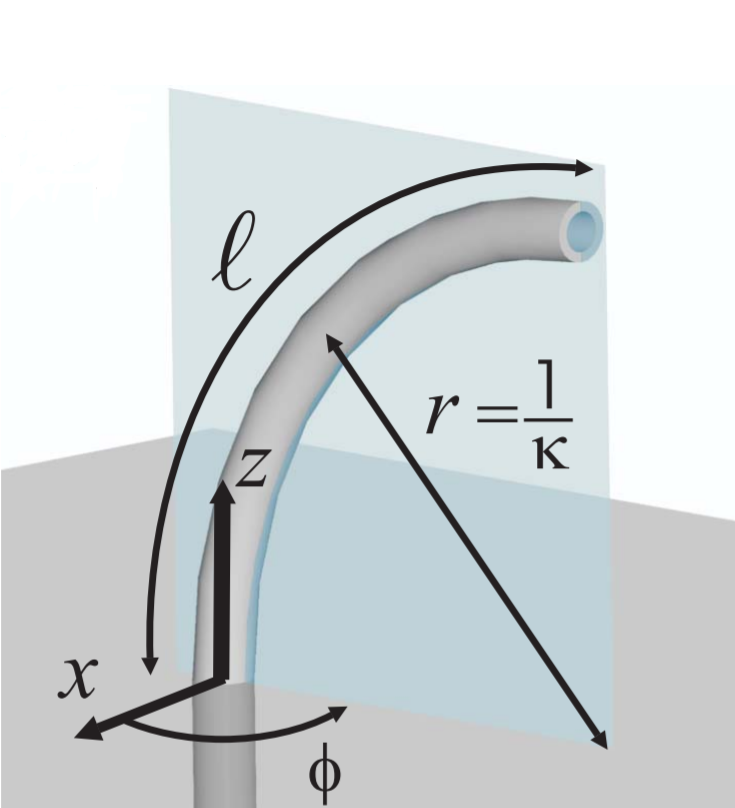
\includegraphics[width=\linewidth]{Figures/Chapter2/ccapproach.png}
              \caption{Schematic drawing of the constant curvature \cite{ccapproach}.}
              \label{fig2:ccapproach}
          \end{figure}
      \end{minipage}
  \end{minipage}

\add{Figure should be adapted with sorotoki one, this looks nicer.}\\


A kinematic description of the actuator is necessary to describe the position in 3D space. Before deriving our kinematic model, we will be briefly discuss constant curvature modeling. Which is a widely used model to describe simplified kinematics of soft actuators \cite{ccapproach},\cite{berkers},\cite{Falkenhahn2015}. A schematic drawing of the constant curvature modelling approach is shown in Figure \ref{fig2:ccapproach}. Although we will not be using this exact methodology, it is important to understand the basics. The constant curvature describes the position of the actuator by three coordinates. Parameter $l$ is the curved length of the actuator measured from the fixed bottom to the tip. Coordinate $\kappa$ expresses the curvature of the actuator. It is assumed that the deformed actuator describes a perfect arc, hence radius $r$ is equal to $\frac{l}{k}$. This allows to write the orientation of the actuator's tip as $\theta = l\kappa$. Lastly, parameter $\phi$ describes the rotation of the actuator with respect to the ground. 

As mentioned, our modelling approach distinguishes itself from the constant curvature model. To describe the kinematics of the soft actuator, a Cosserat beam model is used \cite{Boyer2019}. This beam model can be thought of as a continuous 1-dimensional curve representing the robot's backbone. This backbone is represented in Figure (\ref{fig2:kinematicschematic}) as the black curve. This curve describes the configuration of the soft robot as a function of space and time. To this end, a spatial coordinate  $\sigma \in \mathbb{X}$ within bounded domain $\mathbb{X} \in [0,l] \subset \mathbb{R}$ is introduced. Furthermore, a temporal coordinate $t \in  \mathbb{T}$ with $\mathbb{T} \subseteq \mathbb{R}$ is defined. This allows to describe position $p(\sigma,t) \in \mathbb{R}^3$ and rotation $R(\sigma,t) \in \mathbb{SO}(3)$ 
for any point $\sigma$ and time instance $t$ among the backbone of the soft manipulator by,


\begin{equation}
    g(\sigma,t) = \begin{pmatrix}  R(\sigma,t) & p(\sigma,t) \\ 0_3^\top & 1 \end{pmatrix} \in \mathbb{SE}(3),
    \label{eq2:g}
\end{equation}

where $\mathbb{SE}(3)$ is the Lie group of rigid body transformations in $\mathbb{R}^3$ \cite{Sola2018}. The forward kinematic problem can be found by differentiating (\ref{eq2:g}) with respect to position. This results in the following partial differential equation (PDE), 


\begin{equation}
    \frac{\partial g}{\partial \sigma} = g \hat{\xi} \hspace{10pt} \text{with} \hspace{10pt}  \hat{\xi} = \begin{pmatrix} K_\times & E \\ 0_3^\top & 0 \end{pmatrix} \in  \mathfrak{se}(3)
    \label{eq2:dgdsigma}
\end{equation}

where $\hat{\xi}$ is the space-twist field. Here, $K_\times$ is a skew-symmetric matrix expressing curvature-torsion strain, and $E = [\epsilon_1,\epsilon_2,\epsilon_3]^\top$ a vector containing stretch-shear strain. The entries of $E$ represent  degrees-of-freedom that allow elongation in all three directions. Likewise, the skew-symmetric matrix $K_{\times}$ holds three rotational degrees of freedom.  From this skew-symmetric matrix, vector $K = [\kappa_1,\kappa_2,\kappa_3]^\top$ can be derived \cite{Sola2018}. For the planar robot, it shall be clear that there is one elongation and one rotational degree-of-freedom. In order to include these degrees-of-freedom in the kinematic model, $\epsilon_1$ and $\kappa_2$ will have value 1. All other degrees-of-freedom will take value 0. Defining $\xi(\sigma,t)$ as $[K \hspace{2pt} E]^\top$ results in vector $[0,1,0,1,0,0]^\top$.

To solve the PDE in (\ref{eq2:dgdsigma}), it transformed to an ordinary differential equation (ODE) by exploiting the Galerkin reduction method \cite{Galerkin}. Here, the infinite dimensional system is projected onto a subspace of finite dimension that contains basis elements of the expected solution. By reducing the dimensionality of the system, higher order dynamics are not captured in the model and thus robustness should be taken into account. To transform PDE (\ref{eq2:dgdsigma}), the components of the strain field $\xi(\sigma,t)$ are approximated using a finite amount of shape functions as,

\begin{equation}
    \xi_i(\sigma,t) \approx \sum_{i=1}^N \varphi_i(\sigma)q_i(t) + \xi_{i,0}(\sigma), \hspace{20pt} \forall \sigma \in \mathbb{X}, t \in \mathbb{T},
\end{equation}

in which, $\xi_{i,0}$ corresponds to the undeformed configuration of the robotic manipulator. Additionally, $\{\varphi_i\}_{i \in \mathbb{N}}$ is a set of basis shape functions and $q(t)$ are modal coefficients. These modal coefficients can be thought of as generalized coordinates of the finite-dimensional system. To be clear on this reduction method, integer $N$ is the amount of shape functions used to estimate strain field $\xi(\sigma,t)$. Hence, index $i$ represents the order of the shape function. Several shape functions exist that can be used to approximate the solution. Chebyshev polynomials and Legendre polynomials are a few of those \cite{Galerkin}. Each degree of shape-function gives the model a certain amount of flexibility. Therefore increasing the order of shape-functions allows the model to describe more complex robot configurations. To avoid coupling between shape functions,  it is important that these shape functions are orthogonal. This means that $\int_\mathbb{X} \varphi_i \varphi_j d \sigma = 0$ for any $i \neq j$ and non-zero otherwise. Given this, the $n$-th order strain expansion can be formulated as,

%% maybe write about what shape functions were used, 

\begin{equation}
\begin{aligned}
    \xi(\sigma,t) \cong & \hspace{5pt}  (B_a \otimes [ \varphi_1 \dots \varphi_N ])q(t)\\ = &  \underbrace{ \begin{pmatrix}
    \varphi_1(\sigma) & \dots  & \varphi_N(\sigma) & \dots     & 0      & \dots  &  0 \\
    \vdots    & \ddots & \vdots    & \ddots    & \vdots & \ddots & \vdots \\
    0         & \dots  & 0         & \dots     & \varphi_1(\sigma) & \dots & \varphi_N (\sigma)
    \end{pmatrix}}_{\Phi(\sigma)} \begin{pmatrix} q_1(t) \\ \vdots \\ q_n(t) \end{pmatrix} +  \begin{pmatrix} \xi_{1,0} \\ \vdots \\ \xi_{n,0}   \end{pmatrix}
    \end{aligned},
\label{eq2:xishape}
\end{equation}

where $\Phi \in \mathbb{R}^{m \times n}$ is a shape function matrix in which $n$ is equal to the amount of modal coordinates, and $m$ the amount of active strains, and $B_a \subseteq \text{span}(\mathbb{I}_6)$ a selection matrix of unconstrained strains. For the planar robot, matrix $B_a$ is equal to,

\begin{equation}
    B_a = \begin{bmatrix}
    0 & 1 & 0 & 0 & 0 & 0 \\
    0 & 0 & 0 & 1 & 0 & 0 \\
    \end{bmatrix}^\top
\end{equation}

as is has one free curvature-torsion strain and one stretch-shear strain, This implies that $m = 2$. The amount of shape functions used to approximate a strain affects the value of $n$. Approximating the two strains with a single shape functions gives $n = 2$. 

It should be emphasized that when using a single shape function this Cosserat model reduces to the constant curvature model. In this case the modal coordinates $q(t)$ will be equal to $\kappa$ and $\epsilon$, respectively. 

The forward kinematic problem is programmed in Matlab. Given modal coordinates $q(t)$ and initial conditions at $\sigma = 0$, the actuator position can be calculated. To reduce computation time, the rotation matrix in $g(\sigma,t)$ (\ref{eq2:g}) was reformulated using quaternion formulation \cite{Boyer2019}. This allows to express any rotation by a vector of length 4, instead of 3 by 3 matrix. Therefore $g(\sigma,t)$ can significantly be reduced from 16 entries, to only 7 entries when using quaternion formulation. Any rotation matrix $R(\sigma,t)$ can be rewritten to quaternions by,


\begin{equation}
\frac{\partial}{\partial \sigma}    \begin{pmatrix} Q \\ p \end{pmatrix} = \begin{pmatrix} 2 ||Q||^{-1} A(R(Q)K)Q \\ R(Q)p \end{pmatrix},
\label{eq2:Qp}
\end{equation}

where $Q \in \mathbb{R}^4$ is the quaternion representation of rotation matrix $R$, and $R(Q)$ a function mapping a quaternion to rotation matrix representation, $A$ is a function defined as,


\begin{equation}
    A(K) = \begin{pmatrix} 0 & -K_1 & -K_2 & -K_3 \\ K_1 & 0 & -K_3 & \hspace{8pt}K_2 \\ K_2 & \hspace{8pt}K_3 & 0 & -K_1 \\ K_3 & -K_2 & \hspace{8pt}K_1 & 0 \end{pmatrix},
    \label{eq2:AK}
\end{equation}

where $K_i$ correspond to the entries of $\xi(\sigma,t)$ shown in (\ref{eq2:dgdsigma}). In  (\ref{eq2:Qp}) and (\ref{eq2:AK}) the dependency of $\sigma$ and $t$ has been omitted for the sake of readability.


\section{Dynamic Modelling}


\begin{equation}
    J = Ad_{g(\sigma)^{-1}} \underbrace{\int_0^{L_0} Ad_{g(\sigma)} B_a \Phi(\sigma) d\sigma}_{\Tilde{J}}
\end{equation}


\begin{equation}
    M(q) = \int_0^{L_0} J^\top \mathcal{M}(\sigma) J d \sigma
\end{equation}

\begin{equation}
    T = \frac{1}{2} \int_0^L VM(\sigma)V d\sigma
\end{equation}

where $M = \text{diag}([m_x,m_y,m_z,I_{xx},I_{yy},I_{zz}])$, since it is assumed that $m$ is a point mass it holds that $m_x=m_y=m_z$. And assume we can write V as,

\begin{equation}
    V = J\dot{q},
\end{equation}

Where $J$ can be formulated as,
\begin{equation}
    J = Ad_g^{-1}(\sigma) \int_0^L Ad_g(\sigma) B_a\Phi(\sigma)d\sigma
\end{equation}

Substitution gives,

\begin{equation}
    T = \frac{1}{2}\int_0^L (J(\sigma)\dot{q})^\top M(\sigma) J(\sigma)\dot{q} d\sigma
\end{equation}

This allows to define a mass matrix dependent on modal coordinates $q$ as,

\begin{equation}
    M(q) = J(\sigma)^\top M(\sigma) J(\sigma) 
\end{equation}

The mass matrix is determined using the script below.









\section{Simulation model}

A simplified dynamic model is derived in an effort to capture the dynamics of the soft manipulator. It is assumed that the dynamics of the system can be formulated as, 

\begin{equation}
    M(q)\Ddot{q} + C\dot{q} + K(q)q = u \hspace{10pt} \text{with} \hspace{10pt} u = Hp
\end{equation}

which resembles a non-linear mass-spring-damper system. Here, $M(q)  \in \mathbb{R}^{n\times n}$ is a non-linear mass matrix, $C   \in \mathbb{R}^{n\times n}$ a linear damping matrix, and $K(q)   \in \mathbb{R}^{n\times n}$ a non-linear stiffness matrix. Matrix $H   \in \mathbb{R}^{2\times 2}$ maps input pressure $p$ to forces and moments $u$.

Above dynamic model allows for numeric solving by reformulating the model to a second order state-space formulation as,

\begin{equation}
     \begin{bmatrix} \dot{x}  \end{bmatrix}   =      \begin{bmatrix} O_2 & I_2 \\ -M(q)^{-1}K(q)  & -M(q)^{-1} C \end{bmatrix}      \begin{bmatrix} x \end{bmatrix}  +      \begin{bmatrix} O_2 \\ M(q)^{-1}H   \end{bmatrix}       \begin{bmatrix} p_1\\ p_2   \end{bmatrix} 
\end{equation}

where $x \in \mathbb{R}^{n}$ is the state vector. Assuming the constant curvature approach ($n = 2$) the entries of of $x$ are $ \begin{bmatrix} \epsilon \hspace{3pt} \kappa \hspace{3pt} \dot{\epsilon}  \hspace{3pt} \dot{\kappa}  \end{bmatrix}^{\top}  $










\textbf{Assumptions}
\begin{itemize}
    \item The actuator is symmetrical, curvature equal but negative in when bellow is pressurized
    \item Out of plane motion is negligible small
    \item Constant curvature approach captures the kinematics well when neglecting the effect of gravity 
\end{itemize}
